% ============================================================
% DIAGRAM: RLHF Pipeline (2022)
% ============================================================
% Caption: Figure 7.1: RLHF pipeline for alignment.
%          (Adapted from Ouyang et al., 2022, p. 3)
% ============================================================

\documentclass[tikz,border=10pt]{standalone}
\usepackage{tikz}
\usepackage{amsmath}
\usepackage{amsfonts}

\usetikzlibrary{shapes,arrows,positioning,fit,calc,backgrounds}

\begin{document}

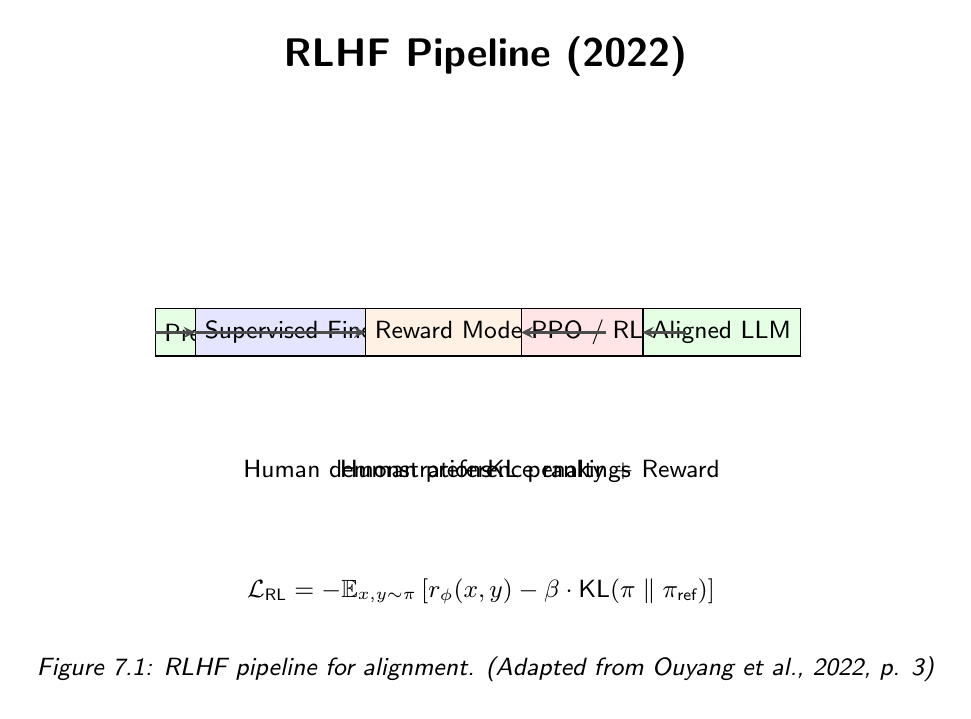
\begin{tikzpicture}[
    block/.style={draw, rectangle, minimum width=1cm, minimum height=0.6cm, fill=blue!10, font=\sffamily\small},
    edge/.style={-stealth, thick, draw=black!70},
    label/.style={font=\sffamily\small},
    title/.style={font=\sffamily\Large\bfseries},
    caption/.style={font=\sffamily\small\itshape},
]

\node[title] at (0, 3.5) {RLHF Pipeline (2022)};

% Pretrained model
\node[block, fill=green!10] (pretrain) at (-3, 0) {Pretrained LLM};

% SFT
\node[block] (sft) at (-1.5, 0) {Supervised Fine-Tuning (SFT)};

% Reward Model
\node[block, fill=orange!10] (rm) at (0, 0) {Reward Model (RM)};

% PPO/RLHF
\node[block, fill=red!10] (ppo) at (1.5, 0) {PPO / RLHF};

% Final model
\node[block, fill=green!10] (final) at (3, 0) {Aligned LLM};

\draw[edge] (pretrain) -- (sft);
\draw[edge] (sft) -- (rm);
\draw[edge] (rm) -- (ppo);
\draw[edge] (ppo) -- (final);

% Labels
\node[align=center, font=\sffamily\small, anchor=north] at (-1.5, -1.5) {Human demonstrations};
\node[align=center, font=\sffamily\small, anchor=north] at (0, -1.5) {Human preference rankings};
\node[align=center, font=\sffamily\small, anchor=north] at (1.5, -1.5) {KL penalty + Reward};

% Objective
\node[align=center, font=\sffamily\small, anchor=north] at (0, -3.0) {
  $\mathcal{L}_{\text{RL}} = -\mathbb{E}_{x,y \sim \pi} \left[ r_\phi(x,y) - \beta \cdot \text{KL}(\pi \parallel \pi_{\text{ref}}) \right]$
};

\node[caption, anchor=north] at (0, -4.0) {
  Figure 7.1: RLHF pipeline for alignment. (Adapted from Ouyang et al., 2022, p. 3)
};

\end{tikzpicture}
\end{document}
